\documentclass{standalone}
\usepackage{tikz}
\usetikzlibrary{patterns, positioning}


\begin{document}
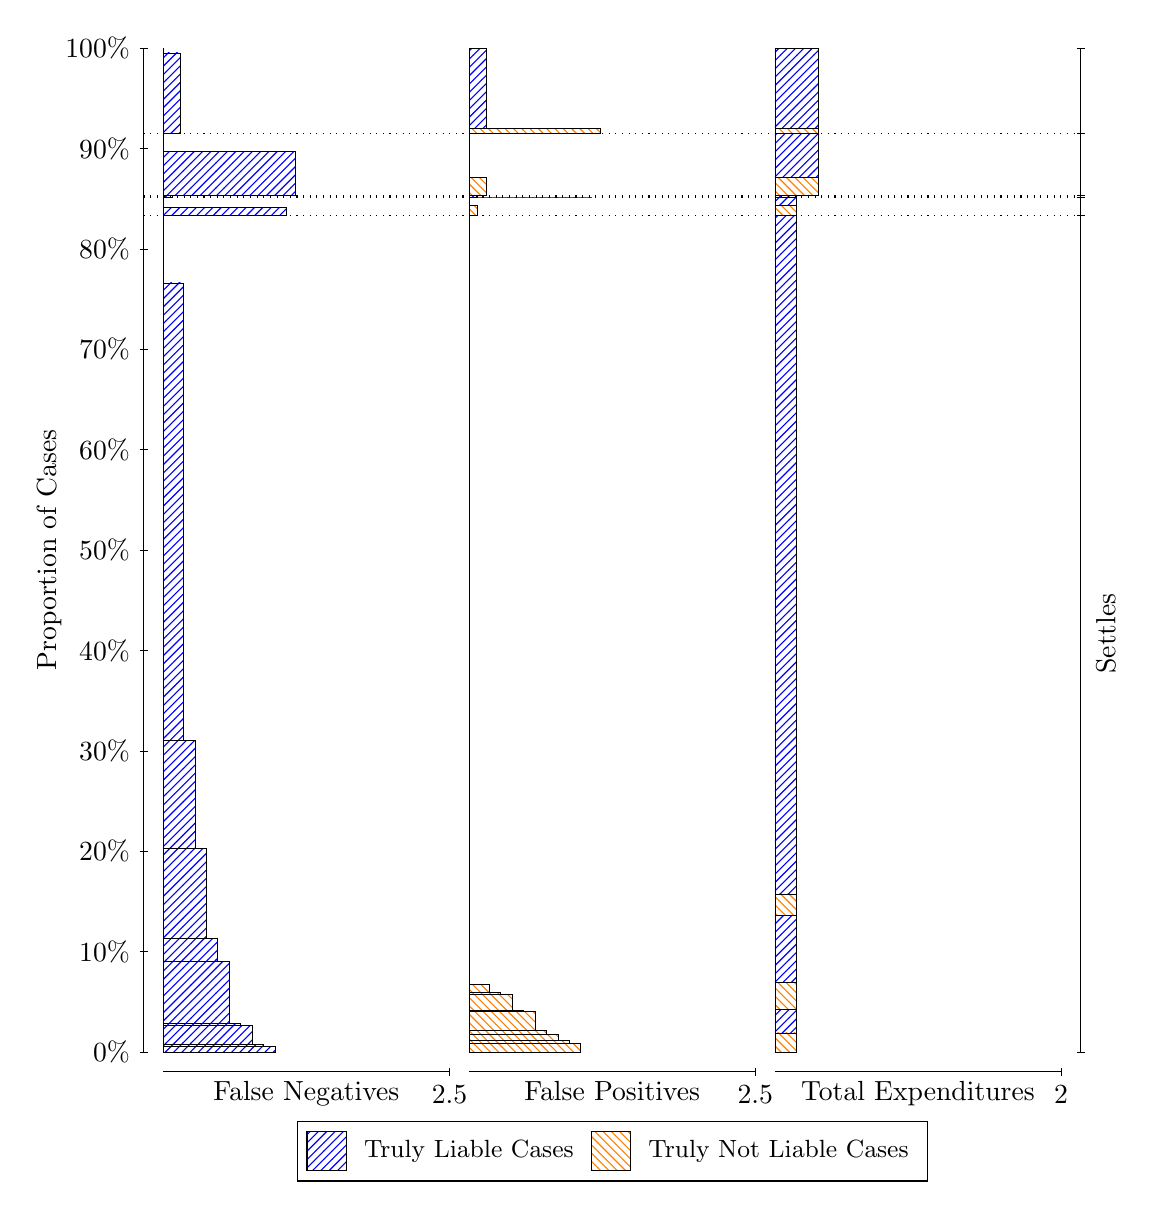
\begin{tikzpicture}
\draw[black, very thin] (1.5,1.75) -- (1.5,14.5);
\node[rotate=90, text=black, anchor=center] at (0.3, 8.125) {Proportion of Cases};
\draw[black, very thin] (1.45,1.75) -- (1.55,1.75);
\node[text=black, anchor=east] at (1.45, 1.75) {0\%};
\draw[black, very thin] (1.45,3.025) -- (1.55,3.025);
\node[text=black, anchor=east] at (1.45, 3.025) {10\%};
\draw[black, very thin] (1.45,4.3) -- (1.55,4.3);
\node[text=black, anchor=east] at (1.45, 4.3) {20\%};
\draw[black, very thin] (1.45,5.575) -- (1.55,5.575);
\node[text=black, anchor=east] at (1.45, 5.575) {30\%};
\draw[black, very thin] (1.45,6.85) -- (1.55,6.85);
\node[text=black, anchor=east] at (1.45, 6.85) {40\%};
\draw[black, very thin] (1.45,8.125) -- (1.55,8.125);
\node[text=black, anchor=east] at (1.45, 8.125) {50\%};
\draw[black, very thin] (1.45,9.4) -- (1.55,9.4);
\node[text=black, anchor=east] at (1.45, 9.4) {60\%};
\draw[black, very thin] (1.45,10.675) -- (1.55,10.675);
\node[text=black, anchor=east] at (1.45, 10.675) {70\%};
\draw[black, very thin] (1.45,11.95) -- (1.55,11.95);
\node[text=black, anchor=east] at (1.45, 11.95) {80\%};
\draw[black, very thin] (1.45,13.225) -- (1.55,13.225);
\node[text=black, anchor=east] at (1.45, 13.225) {90\%};
\draw[black, very thin] (1.45,14.5) -- (1.55,14.5);
\node[text=black, anchor=east] at (1.45, 14.5) {100\%};

\draw[black, very thin] (13.4,1.75) -- (13.4,14.5);
\draw[black, very thin] (13.35,1.75) -- (13.45,1.75);
\node[anchor=west] at (13.35, 1.75) {};
\draw[black, very thin] (13.35,12.377) -- (13.45,12.377);
\node[anchor=west] at (13.35, 12.377) {};
\draw[black, very thin] (13.35,12.608) -- (13.45,12.608);
\node[anchor=west] at (13.35, 12.608) {};
\draw[black, very thin] (13.35,12.632) -- (13.45,12.632);
\node[anchor=west] at (13.35, 12.632) {};
\draw[black, very thin] (13.35,13.417) -- (13.45,13.417);
\node[anchor=west] at (13.35, 13.417) {};
\draw[black, very thin] (13.35,14.5) -- (13.45,14.5);
\node[anchor=west] at (13.35, 14.5) {};

\draw[black, very thin, pattern color=blue, pattern=north east lines] (1.75,1.75) rectangle (3.167,1.8189);
\draw[black, very thin, pattern color=blue, pattern=north east lines] (1.75,1.8189) rectangle (3.0217,1.8512);
\draw[black, very thin, pattern color=blue, pattern=north east lines] (1.75,1.8512) rectangle (2.8763,2.0868);
\draw[black, very thin, pattern color=blue, pattern=north east lines] (1.75,2.0868) rectangle (2.731,2.1147);
\draw[black, very thin, pattern color=blue, pattern=north east lines] (1.75,2.1147) rectangle (2.5857,2.8977);
\draw[black, very thin, pattern color=blue, pattern=north east lines] (1.75,2.8977) rectangle (2.4403,3.193);
\draw[black, very thin, pattern color=blue, pattern=north east lines] (1.75,3.193) rectangle (2.295,4.3346);
\draw[black, very thin, pattern color=blue, pattern=north east lines] (1.75,4.3346) rectangle (2.1497,5.7108);
\draw[black, very thin, pattern color=blue, pattern=north east lines] (1.75,5.7108) rectangle (2.0043,11.517);
\draw[black, very thin, pattern color=orange, pattern=north west lines] (1.75,11.517) rectangle (1.75,12.377);
\draw[black, very thin, pattern color=blue, pattern=north east lines] (1.75,12.377) rectangle (3.3123,12.48);
\draw[black, very thin, pattern color=orange, pattern=north west lines] (1.75,12.48) rectangle (1.75,12.608);
\draw[black, very thin, pattern color=blue, pattern=north east lines] (1.75,12.608) rectangle (1.859,12.632);
\draw[black, very thin, pattern color=orange, pattern=north west lines] (1.75,12.632) rectangle (1.75,12.632);
\draw[black, very thin, pattern color=blue, pattern=north east lines] (1.75,12.632) rectangle (3.4213,13.192);
\draw[black, very thin, pattern color=orange, pattern=north west lines] (1.75,13.192) rectangle (1.75,13.417);
\draw[black, very thin, pattern color=blue, pattern=north east lines] (1.75,13.417) rectangle (1.968,14.438);
\draw[black, very thin, pattern color=orange, pattern=north west lines] (1.75,14.438) rectangle (1.75,14.5);
\draw[black, very thin, pattern color=orange, pattern=north west lines] (5.6333,1.75) rectangle (7.0503,1.8546);
\draw[black, very thin, pattern color=orange, pattern=north west lines] (5.6333,1.8546) rectangle (6.905,1.8923);
\draw[black, very thin, pattern color=orange, pattern=north west lines] (5.6333,1.8923) rectangle (6.7597,1.9765);
\draw[black, very thin, pattern color=orange, pattern=north west lines] (5.6333,1.9765) rectangle (6.6143,2.0245);
\draw[black, very thin, pattern color=orange, pattern=north west lines] (5.6333,2.0245) rectangle (6.469,2.268);
\draw[black, very thin, pattern color=orange, pattern=north west lines] (5.6333,2.268) rectangle (6.3237,2.2828);
\draw[black, very thin, pattern color=orange, pattern=north west lines] (5.6333,2.2828) rectangle (6.1783,2.4781);
\draw[black, very thin, pattern color=orange, pattern=north west lines] (5.6333,2.4781) rectangle (6.033,2.5113);
\draw[black, very thin, pattern color=orange, pattern=north west lines] (5.6333,2.5113) rectangle (5.8877,2.6097);
\draw[black, very thin, pattern color=blue, pattern=north east lines] (5.6333,2.6097) rectangle (5.6333,12.377);
\draw[black, very thin, pattern color=orange, pattern=north west lines] (5.6333,12.377) rectangle (5.7423,12.505);
\draw[black, very thin, pattern color=blue, pattern=north east lines] (5.6333,12.505) rectangle (5.6333,12.608);
\draw[black, very thin, pattern color=orange, pattern=north west lines] (5.6333,12.608) rectangle (7.1957,12.608);
\draw[black, very thin, pattern color=blue, pattern=north east lines] (5.6333,12.608) rectangle (5.7423,12.632);
\draw[black, very thin, pattern color=orange, pattern=north west lines] (5.6333,12.632) rectangle (5.8513,12.857);
\draw[black, very thin, pattern color=blue, pattern=north east lines] (5.6333,12.857) rectangle (5.6333,13.417);
\draw[black, very thin, pattern color=orange, pattern=north west lines] (5.6333,13.417) rectangle (7.3047,13.478);
\draw[black, very thin, pattern color=blue, pattern=north east lines] (5.6333,13.478) rectangle (5.8513,14.5);
\draw[black, very thin, pattern color=orange, pattern=north west lines] (9.5167,1.75) rectangle (9.7892,1.9932);
\draw[black, very thin, pattern color=blue, pattern=north east lines] (9.5167,1.9932) rectangle (9.7892,2.289);
\draw[black, very thin, pattern color=orange, pattern=north west lines] (9.5167,2.289) rectangle (9.7892,2.631);
\draw[black, very thin, pattern color=blue, pattern=north east lines] (9.5167,2.631) rectangle (9.7892,3.4829);
\draw[black, very thin, pattern color=orange, pattern=north west lines] (9.5167,3.4829) rectangle (9.7892,3.7574);
\draw[black, very thin, pattern color=blue, pattern=north east lines] (9.5167,3.7574) rectangle (9.7892,12.377);
\draw[black, very thin, pattern color=orange, pattern=north west lines] (9.5167,12.377) rectangle (9.7892,12.505);
\draw[black, very thin, pattern color=blue, pattern=north east lines] (9.5167,12.505) rectangle (9.7892,12.608);
\draw[black, very thin, pattern color=orange, pattern=north west lines] (9.5167,12.608) rectangle (9.7892,12.608);
\draw[black, very thin, pattern color=blue, pattern=north east lines] (9.5167,12.608) rectangle (9.7892,12.632);
\draw[black, very thin, pattern color=orange, pattern=north west lines] (9.5167,12.632) rectangle (10.062,12.857);
\draw[black, very thin, pattern color=blue, pattern=north east lines] (9.5167,12.857) rectangle (10.062,13.417);
\draw[black, very thin, pattern color=orange, pattern=north west lines] (9.5167,13.417) rectangle (10.062,13.478);
\draw[black, very thin, pattern color=blue, pattern=north east lines] (9.5167,13.478) rectangle (10.062,14.5);
\draw[black, dotted] (1.5,12.377) -- (13.4,12.377);
\draw[black, dotted] (1.5,12.608) -- (13.4,12.608);
\draw[black, dotted] (1.5,12.632) -- (13.4,12.632);
\draw[black, dotted] (1.5,13.417) -- (13.4,13.417);
\draw[black, very thin] (1.75,1.5) -- (5.3833,1.5);
\node[text=black, anchor=north] at (3.5667, 1.5) {False Negatives};
\draw[black, very thin] (5.3833,1.45) -- (5.3833,1.55);
\node[text=black, anchor=north] at (5.3833, 1.45) {2.5};

\draw[black, very thin] (5.6333,1.5) -- (9.2667,1.5);
\node[text=black, anchor=north] at (7.45, 1.5) {False Positives};
\draw[black, very thin] (9.2667,1.45) -- (9.2667,1.55);
\node[text=black, anchor=north] at (9.2667, 1.45) {2.5};

\draw[black, very thin] (9.5167,1.5) -- (13.15,1.5);
\node[text=black, anchor=north] at (11.333, 1.5) {Total Expenditures};
\draw[black, very thin] (13.15,1.45) -- (13.15,1.55);
\node[text=black, anchor=north] at (13.15, 1.45) {2};

\node[text=black, centered, rotate=90] at (13.72, 7.0634) {Settles};





\draw (7.449999999999999,1.5) node[draw=none] (baseCoordinate) {};
\begin{scope}[align=center]
        \matrix[scale=0.5, draw=black, below=0.5cm of baseCoordinate, nodes={draw}, column sep=0.1cm]{
            \node[rectangle, draw, minimum width=0.5cm, minimum height=0.5cm, pattern color=blue, pattern=north east lines] {}; &
            \node[draw=none, font=\small, text=black] (B) {Truly Liable Cases}; &
            \node[rectangle, draw, minimum width=0.5cm, minimum height=0.5cm, pattern color=orange, pattern=north west lines] {}; &
            \node[draw=none, font=\small, text=black] (B) {Truly Not Liable Cases}; \\
            };
\end{scope}

\end{tikzpicture}
\end{document}